\begin{figure}[htbp]
\section*{ ZMYM3}
\centering
\begin{subfigure}[b]{0.95\textwidth}
\centering
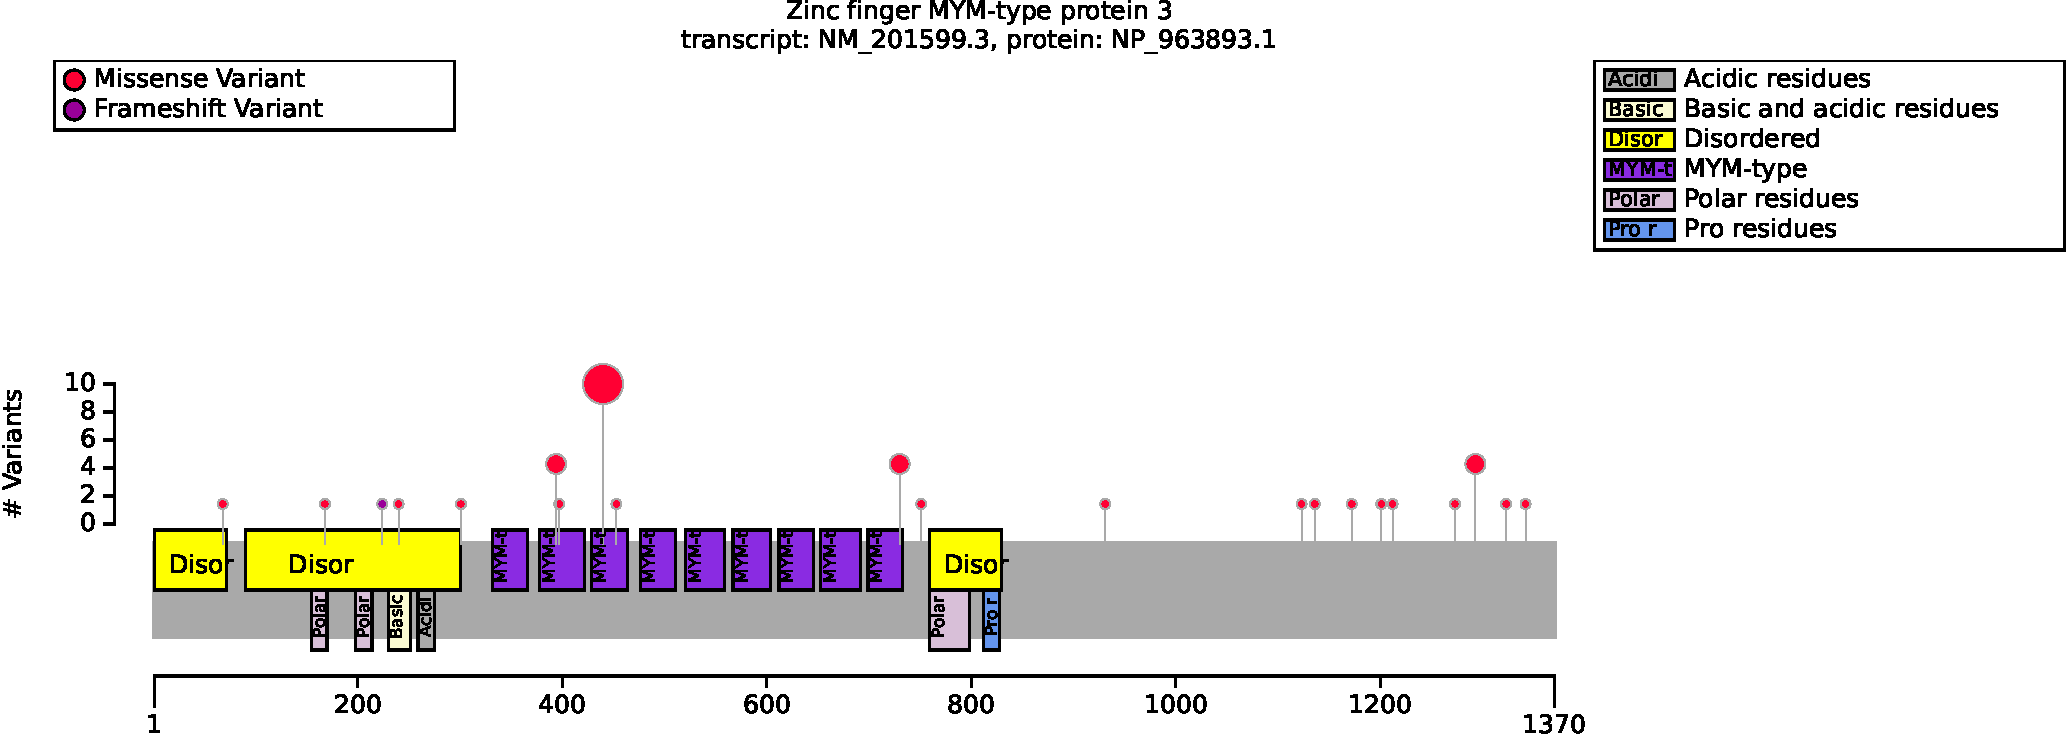
\includegraphics[width=\textwidth]{ img/ZMYM3_protein_diagram.pdf} 
\captionsetup{justification=raggedright,singlelinecheck=false}
\caption{Distribution of variants in ZMYM3}
\end{subfigure}
\vspace{2em}

\begin{subfigure}[b]{0.95\textwidth}
\centering
\resizebox{\textwidth}{!}{
\begin{tabular}{llllrr}
\toprule
HPO term & R441 & other & p-value & adj. p-value\\
\midrule
Cupped ear [HP:0000378] & 7/10 (70\%) & 1/23 (4\%) & $2.02\times 10^{-4}$ & 0.012\\
\bottomrule
\end{tabular}
}
\captionsetup{justification=raggedright,singlelinecheck=false}
\caption{Fisher Exact Test performed to compare HPO annotation frequency with respect to R441 and other. Total of 60 tests were performed. }
\end{subfigure}
\vspace{2em}
\begin{subfigure}[b]{0.95\textwidth}
\centering
\resizebox{\textwidth}{!}{
\begin{tabular}{llllrr}
\toprule
Genotype (A) & Genotype (B) & total tests performed & significant results\\
\midrule
N term & other & 60 & 0\\
\bottomrule
\end{tabular}
}
\captionsetup{justification=raggedright,singlelinecheck=false}
\caption{Fisher Exact Test performed to compare HPO annotation frequency with respect to genotypes. }
\end{subfigure}

\vspace{2em}

\caption{ The cohort comprised 33 individuals (3 females, 30 males). 1 of these individuals were reported to be deceased. A total of 78 HPO terms were used to annotate the cohort. Disease diagnosis: Intellectual developmental disorder, X-linked 112 (OMIM:301111).  A total of 22 unique variant alleles were found in \textit{ZMYM3} (transcript: \texttt{NM\_201599.3}, protein id: \texttt{NP\_963893.1}). No analysis of ZMYM3 genotype phgenotype correlation was presented in the two studies on ZMYM3 variants study to be published to date \cite{PMID_24721225,PMID_36586412}.}
\end{figure}
